\documentclass[a4paper,12pt]{article}
\usepackage{graphicx} 			% Para insertar imagenes
\usepackage{indentfirst} 	% Para sangrar párrafos después de secciones
\setlength{\parindent}{1.5cm} 	% Sangría de 1.5 cm
\usepackage{minted} 	% Para insertar código 
\usepackage{float}
\usepackage[spanish, es-tabla]{babel}
\usepackage{tcolorbox} % Para secciones en destacado
\usepackage{amsmath}
\usepackage{amssymb}
\usepackage{hyperref} % Para los enlaces
\usepackage{tcolorbox} % Para secciones en destacado


\title{Práctica 1. Patrones de diseño. }
\author{Javier Ortega Medina}
\author{Ángel Rodríguez Faya}
\date{22 de marzo de 2026}

\begin{document}
	
	% --- PÁGINA 1: LA PORTADA ---
	\begin{titlepage}
		\centering
		\vspace*{1cm}
		
		{\huge\bfseries Práctica 1. Patrones de diseño.}
		\vspace{1.5 cm}
		
		{\Large Desarrollo de Software. Grupo DS-3. \par}
		\vspace{0.25cm}
		{\Large Grado en Ingeniería Informática \par}
		\vspace{0.25cm}
		{\Large Curso 2025-2026.\par}
		\vspace{0.25cm}
		{\Large ETSIIT. Universidad de Granada.\par}
		\vspace{1 cm}
		
		\noindent % Evita la sangría para que aproveche todo el ancho
		\begin{minipage}[c]{0.55\textwidth}
			% La imagen ocupa el 100% del ancho DE ESTA CAJA (no de la hoja)
			
\includegraphics[width=\linewidth]{../memoria/imagenes_necesarias/Logotipo_ETSIIT_Horizontal_color.png}
		\end{minipage}% <--- Este % es importante para que no añada espacios extra
		\hfill % Rellena el espacio en medio empujando las cajas a los extremos
		\begin{minipage}[c]{0.40\textwidth}
			\raggedleft % Alinea esta imagen a la derecha dentro de su caja
			
\includegraphics[width=\linewidth]{../memoria/imagenes_necesarias/UGR-LOGO-color.png}
		\end{minipage}
		
		\vspace{0.5 cm}
		
		{\large\bfseries Autores: \par}
		{\large Javier Ortega Medina \par}
		{\large Ángel Rodríguez Faya \par}
		\vspace{0.5cm}
		
		{\large\bfseries Profesor: \par}
		{\large Alberto Jesús Durán López\par}
		\vspace{1 cm}
		
		{\large\bfseries Fecha de entrega: \par}
		{\large 22 de marzo de 2026\par}
		
	\end{titlepage}
	% El entorno 'titlepage' hace el salto de página automáticamente al cerrar.
	
	% --- PÁGINA 2: EL ÍNDICE ---
	\tableofcontents
	\newpage % <--- Fuerza el salto a la página 3
	
	% --- RESTO DE PÁGINAS:
	
	% Forzamos el contador a -1 justo antes de la primera sección.
	% Esto es para que las secciones comiencen por 0
	\setcounter{section}{-1}
	
	\section{Introducción}
		El objetivo de esta práctica es familiarizarnos con los patrones de diseño creacionales y estructurales, que hemos visto en el Tema 1 de esta asignatura. Para ello, hemos desarrollado 4 ejercicios los cuáles se podrían considerar como mini-proyectos que hacen uso del paradigma de programación orientada a objetos (POO). Además, están implementados en distintos lenguajes de programación como Java, Python y Ruby. \newline
		
		Algunas anotaciones a tener en cuenta sobre la practica:
		
		\begin{itemize}
			\item El enlace al repositorio de GitHub de las prácticas de Desarrollo de Software es: \url{https://github.com/AngelRodriguezFaya/practicas_desarrollo_de_software} 
			
			\item Cada ejercicio tiene su propio directorio. Dentro de cada directorio encontramos otros dos directorios. Uno contiene el \textbf{código fuente del ejercicio}, el otro contiene \textbf{los diagramas de clase en UML}. \textbf{Si las imágenes de los diagramas de clase no se visualizan correctamente en este documento (aunque como tienen una calidad de 600 DPI, si se hace \textit{zoom} se pueden ver correctamente) , siempre podemos ir a este directorio y ahí nos encontraremos la misma imagen.}
			
			\item La práctica la hemos desarrollado en nuestros ordenadores personales, utilizando para ello:
				\begin{itemize}
					\item \textbf{Sistemas Operativos:} \texttt{Ubuntu 24.04 LTS} y \texttt{Debian 13 trixie}.
					
					\item \textbf{Entornos de desarrollo: } \texttt{Visual Studio Code} para Python, \texttt{IntelliJ Ultimate} para Java y \texttt{RubyMine} para Ruby.
				\end{itemize}
		\end{itemize}
		
		\newpage
	
	\section{Ejercicio 1. Patrón Factoria Abstracta en Java.}
		En este ejercicio teníamos que implementar  un sistema que simulase dos partidas multijugadores y simultáneas, con el mismo númeero de jugadores y a determinar en tiempo de ejecución (lo introduce el usuario al principio). Para ello debíamos utilizar hebras, haciendo uso de la interfaz \texttt{Runnable}. 
		
		Las partidas tienen algunas características como: las modalidades (Competitiva y Casual), la tasa de abandonos (en el caso de la partida Competitiva sería de un 20\% del total de jugadores mientras que para la modalidad Casual sería de un 10\% del total de jugadores), ambas partidas tienen una duración de 60 segundos y los abandonos de jugadores se producen al mismo tiempo.
		
		Para este ejercicio tenemos que implementar el patrón Factoría Abstracta, que es un patrón creacional. Los \textbf{patrones creacionales} son aquellos que implmenetan mecanismos de creación de objetos aumentando la flexibilidad y reutilización del código. El \textbf{patrón Factoría Abstracta} nos permite producir familias de objetos relacionados y dependientes sin especificar sus clases concretas, es decir, funciona como una \textit{fábrica de fábricas}, donde se encapsula la creación de los productos y se garantiza la compatibilidad entre ellos. Eso es justo lo que necesitamos para este ejercicio pues necesitamos crear partidas y jugadores de la misma modalidad, y no mezclarlos.
		
		Veamos los elementos del proyecto y que función cumplen cada uno de ellos en relación con el patrón de diseño impuesto:
		
		\subsection{Descripción de elementos del proyecto.}
			\begin{itemize}
				\item \textbf{Clase \texttt{Jugador}}. Esta clase es abstracta. Tiene un único atributo que es un entero que hace de indentificador del jugador que encapsula.

				\item \textbf{Clase \texttt{JugadorCompetitivo}}. Hereda de la clase padre: \texttt{Jugador}. Modela un jugador de la modalidad de partida Competitiva. 
				
				\item \textbf{Clase \texttt{JugadorCasual}}. Hereda de la clase padre:\texttt{Jugador}. Modela un jugador de la modalidad de partida Casual.
				
				\item \textbf{Clase \texttt{Partida}}.Es una clase abstracta e implementa la interfaz \texttt{Runnable} de la que hablamos anteriormente, es necesaria para poder crear hebras (que en realidad serán partidas ejecutándose de forma concurrente). Esta clase modela una partida de nuestro programa y es abstracta porque hay dos tipos de partidas (que serán sus clases hijas y las que implementen los métodos abstractos que declara). Esta clase tiene las siguientes carácteristicas:
				\begin{itemize}
					\item Tiene una colección de objetos de la clase \texttt{Jugador}, que serán los jugadores que tiene la partida. 
					
					\item Además implementa los correspondientes métodos para añadir jugadores a la partida y eliminarlos.
					
					\item Los jugadores los elimina de forma aleatoria, viene implementado en la función \mintinline{Java}|eliminarJugadorRandom()|. También se pueden eliminar un número de jugadores determinado, haciendo uso de la función \mintinline{Java}|eliminarVariosJugadores(int numEliminados)|, que llama  a la función anterior tantas veces como indique \textit{numEliminados}, aunque deberá de ser menor que el número de jugadores total de la partida.
					
					\item Implementa el método \mintinline{Java}|run()| de la interfaz \texttt{Runnable}, que es el método que le indica al hilo lo que debe de hacer, simulando el transcurso de la partida. Lo que hace es: espera (o duerme) la mitad del tiempo de la partida, después elimina tantos jugadores como toquen (que ya hemos visto que el porcentaje varía dependiendo del tipo de partida), después duerme el tiempo restante y finalmente termina la partida.
					
					\item Define la cabecera de los dos métodos abstractos \mintinline{Java}|getModalidadPartida()| y \mintinline{Java}|getPorcentajeAbandono()| que deberán de implementar las clases hijas dependiendo de la modalidad de la partida.
				\end{itemize}
				
				\item \textbf{Clase \texttt{PartidaCompetitiva}}. Hereda de la clase:\texttt{Partida}. Modela una  partida de la modalidad Competitiva (con un 20\% de abandonos) e implementa los dos métodos abstractos de la clase padre.
				
				\item \textbf{Clase \texttt{PartidaCasual}}. Hereda de la clase:\texttt{Partida}. Modela una  partida de la modalidad Casual (con un 10\% de abandonos) y también implementa los dos métodos abstractos de la clase padre.
				
				\item \textbf{Interfaz \texttt{FactoriaPartidaYJugador}}.Es una interfaz que define la cabecera de los métodos \mintinline{Java}|crearPartida(int numJugadores)| y \mintinline{Java}|crearJugador(int id)| que crean una instancia de Partida y otra de Jugador, respectivamente. De esta forma ( y con las clases que implementan esta interfaz y que veremos a continuación) conseguimos crear objetos \textbf{del mismo tipo} y \textbf{sin conocer sus clases concretas}.
				
				\item \textbf{Clase \texttt{FactoriaCompetitiva}}.Esta clase implemnenta la interfaz 
				
				\texttt{FactoriaPartidaYJugador}. Puede \textbf{crear partidas o jugadores de la modalidad Competitiva}.
				
				\item \textbf{Clase \texttt{FactoriaCasual}}.Esta clase implemnenta la interfaz 
				
				\texttt{FactoriaPartidaYJugador}. Puede \textbf{crear partidas o jugadores de la modalidad Casual}.
				
				\item \textbf{Clase \texttt{Cliente}}. Esta clase incluye el programa principal (el \texttt{main}). Hace uso de la \texttt{FactoriaPartidaYJugador} y de \texttt{Partida}. En el programa principal hacemos lo siguiente:
				\begin{enumerate}
					\item \textbf{Creamos una \texttt{Factoria Competitiva} y una \texttt{Factoria Casual}.}
					
					\item Pedimos al usuario que \textbf{ingrese el número de jugadores} de la partida. No continuamos hasta que no sea un número de jugadores válido.
					
					\item Creamos las \textbf{partidas} (Competitiva y Casual)  haciendo uso de las Factorias que creamos en el paso nº1.
					
					\item Creamos los \textbf{jugadores} Competitivos y Casual haciendo uso de nuevo, de la Factoria Competitiva y Factoria Casual respectivamente. Añadimos cada jugador a su partida correspondiente, haciendo uso del método que definimos en la clase \texttt{Plantilla} .
					
					\item \textbf{Declaramos los hilos} sobre las partidas.
					
					\item  \textbf{Arrancamos los hilos}, haciendo uso del método \mintinline{Java}|start()|
					
					\item Hacemos un \texttt{try-catch} para \textbf{esperar a que terminen los hilos} y capturar alguna excepción de que se haya interrumpido el hilo (si es que la hay).
					
					\item El programa finaliza.
				
				\end{enumerate}
			
			\end{itemize}
			
			\subsection{Diagrama de clases en UML.}
				El diagrama de clases formado por los elementos de este proyecto/ejercicio, los cuáles hemos descrito en el apartado anterior, es:  
				
				\begin{figure}[H]
					\centering
					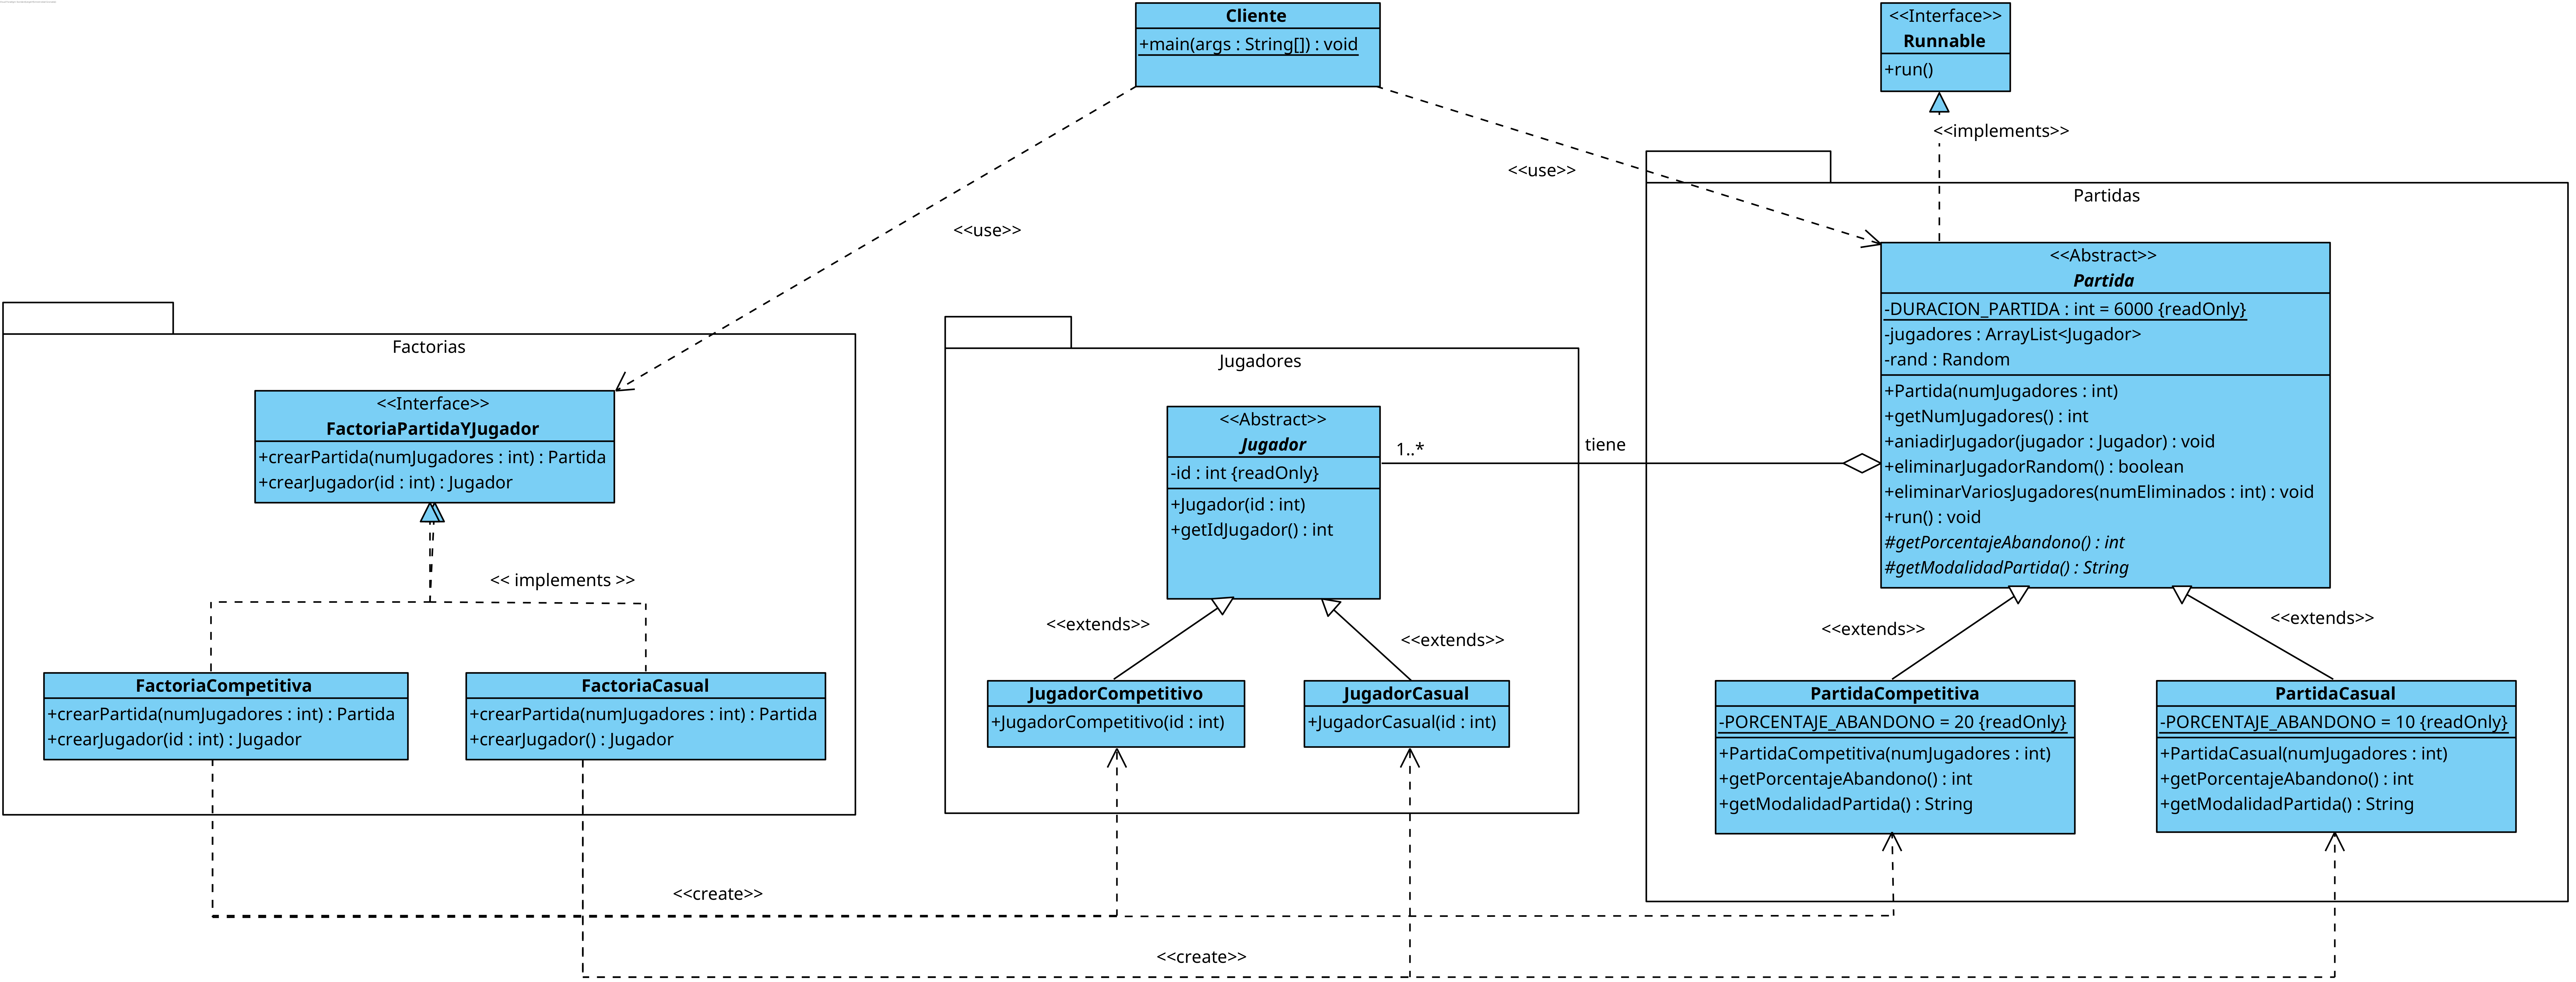
\includegraphics[width=1\linewidth]{../Ejercicio_1_Patron_Factoria_Abstracta_en_Java/diagrama_de_clases/DC EJ1 P1 DS.png}
					\caption{Diagrama de clases del ejercicio 1: Patrón Factoria Abstracta en Java. }
					\label{fig:dc_ej1}
				\end{figure}
			
			\subsection{Ejemplo de compilación y ejecución.}
				Para ejecutar este programa hay dos formas: 
				\begin{enumerate}
					\item Compilando y ejecutando directactemnete el \texttt{Cliente.java} desde \texttt{IntelliJ}, con tan sólo pulsar el bóton de 'Play'. \textbf{(Opción recomendada)}
					
					\item Compilando y ejecutando desde la terminal. 
					\begin{itemize}
						\item Para compilar ejecutamos el siguiente comando:
							\begin{center}
								\fbox{\texttt{\$ mkdir -p bin \&\& javac -d bin -sourcepath src src/Cliente.java}}
							\end{center}
						
						\item Para ejecutar el programa ejecutamos el siguiente comando:
							\begin{center}
								\fbox{\texttt{\$ java -cp bin Cliente }}
							\end{center}
						
					\end{itemize}
				\end{enumerate}
			
			A continuación, mostramos una captura de pantalla sobre un ejemplo de ejecución con \textbf{20 jugadores en la partida}
			
			\begin{figure}[H]
				\centering
				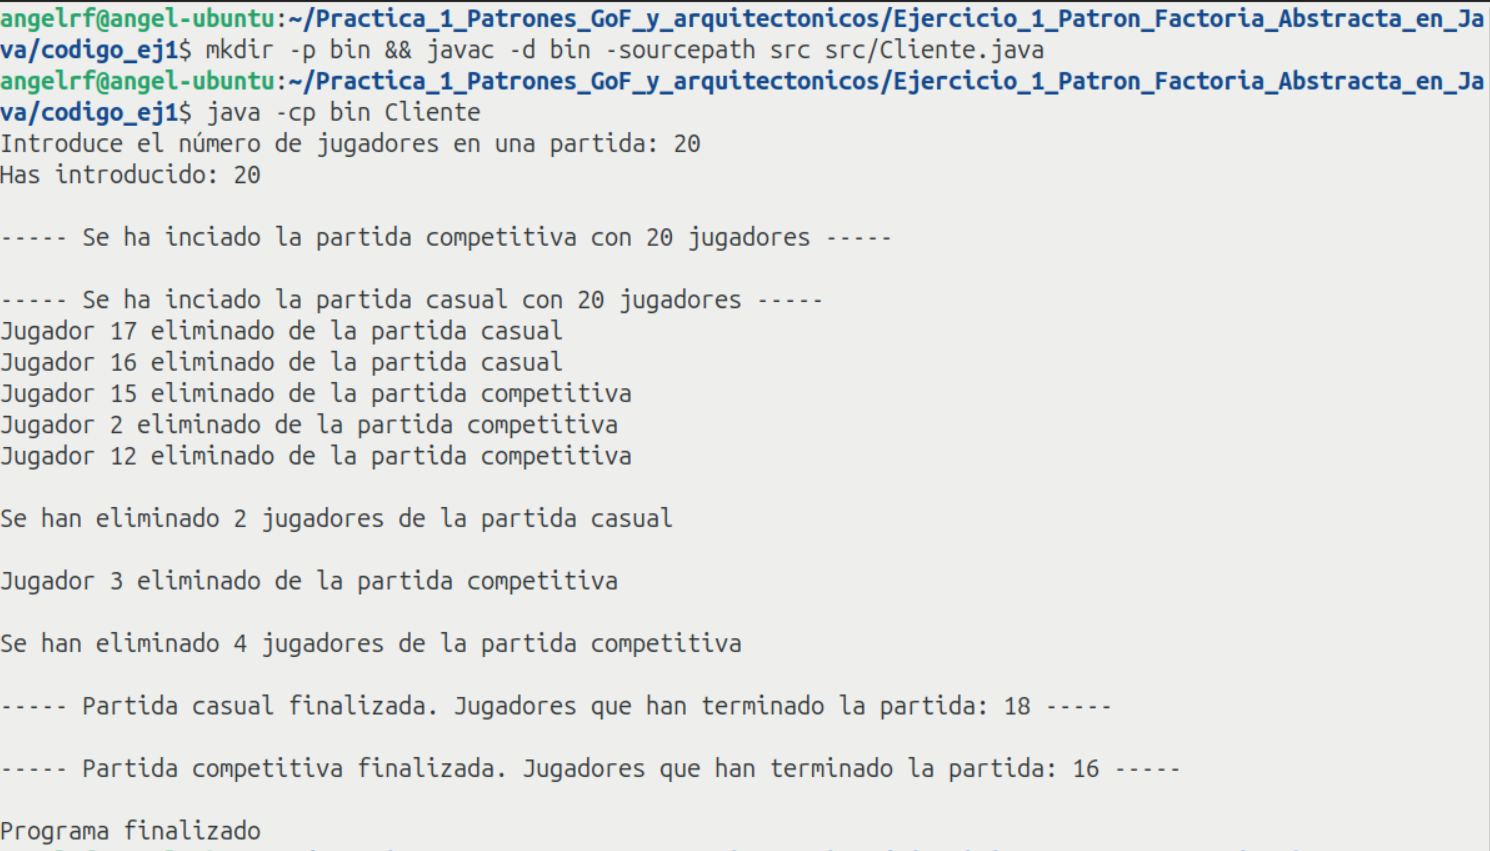
\includegraphics[width=1\linewidth]{./imagenes_necesarias/ejemplo_ej1.png}
				\caption{Ejemplo de ejecución del ejercicio 1 con 20 jugadores en cada partida.}
				\label{fig:ejemplo_ej1}
			\end{figure}
		
		
		Como podemos observar en los resultados de la ejecución, en la partida Casual han abandonando 2 jugadores (el 10\% de 20) y en la Competitiva han abandonado 4 jugadores (20\% de 20). Los \texttt{identificadores} de los jugadores se repiten entre partidas pero debemos de tener en cuenta que son partidas independientes que se ejecutan de forma concurrente, es por eso que aunque haya dos jugadores con el id = 5, por ejemplo, son dos jugadores totalmente distintos pues cada uno está en una partida distinta.
		
		\newpage
	
	\section{Ejercicio 2. Patrón Decorador en Python.}
		El objetivo de este ejercicio es aplicar el patrón Decorador para que al ejecutar el \texttt{main} se realice un resumen de un texto, luego se traduzca de inglés a español y por último se imprima un análisis de sentimientos (calificado con estrellas). 
		El \textbf{patrón Decorador} es un patrón estructural. Los \textbf{patrones estructurales} explican cómo ensamblar objetos y clases en estructuras más grandes y complejas, a la vez que se mantiene la flexibilidad y eficiencia de estas estructuras. 
		\subsubsection*{¿Cuál es la clave detrás del Patrón Decorador en este ejercicio?}

		Este patrón nos permite encadenar diferentes funcionalidades (resumen, traducción, etc.) envolviendo un objeto base con distintas capas o decoradores.

		En nuestra implementación, el objeto \texttt{BasicLLM} es la base que se envuelve primero con el decorador de traducción y posteriormente con el decorador de análisis de sentimiento.

		De esta forma, cuando invocamos al método \texttt{generate\_summary}, la llamada se propaga desde el decorador más externo hacia el objeto base, ejecutándose en cascada. Primero se genera el resumen original, luego se traduce y finalmente se analiza su sentimiento.

		Cada decorador añade su comportamiento sin modificar el código del objeto base, permitiendo una composición flexible y dinámica de funcionalidades.
		
		Vamos a ir viendo cada clase y comentando lo más relevante de ella, además de explicar que función cumple dentro del patrón que se implementa en este ejercicios.
		
		\subsection{Descripción de elementos del proyecto.}
			\begin{itemize}
				\item \textbf{Clase \texttt{LLM}}. Se trata de una clase abstracta para los modelos de lenguaje (LLM) que se utilizarán para generar resúmenes. Define el método común \mintinline{python}| generate_summary(self, text: str) | que deben implementar todos los componentes.
				
				\item \textbf{Clase \texttt{BasicLLM}}: realiza la funcionalidad base. Se encarga mediante \mintinline{python}| generate_summary | de generar un resumen del texto (\texttt{String}) original. 
				La dinámica que seguimos para generar el resumen y qué luego aplicaremos también para los decoradores es:
				\begin{enumerate}
					\item Necesitamos una \texttt{url} de \texttt{HuggingFace} que usaremos. No es fija sino que depende de la variable que pasemos (el tipo de modelo que queramos usar), en nuestro caso definido en el archivo \texttt{config.json}.
					
					\item  Necesitamos un \textit{token} para autenticarnos (también el \texttt{.json}), para ello usamos las cabeceras. 
					
					\item El \texttt{payload}, no es más que el texto que queremos resumir.
					
					\item La petición \texttt{POST}. Hacemos un \texttt{request.post} a \texttt{HuggingFace}.
					
					\item Por último, convertimos la respuesta de \texttt{json} para poder imprimirlo por pantalla. (Incluimos el manejo de posibles errores de recepción del \texttt{JSON}).
				\end{enumerate}
				
				\item \textbf{Clase \texttt{LLMDecorator}}: clase base de los decoradores, que contiene una referencia a un objeto \texttt{LLM} y delega en él la ejecución.
				
				\item \textbf{Clase \texttt{TranslationDecorator}}: siguiendo la dinámica de antes, aplicamos la lógica del decorador traductor. Simplemente se encarga de añadir la capa de la traducción del texto resumido, lo traduce de inglés a español.
				
				\item \textbf{Clase \texttt{SentimentDecorator}}: igual que el Traductor, pero añade la capa de hacer un \textit{rating} (con estrellas) acerca de los sentimientos que transmite ese texto. 			
			\end{itemize}
			
			El archivo \texttt{config.json} queda de la siguiente forma:
			\begin{figure}[H]
				\centering
				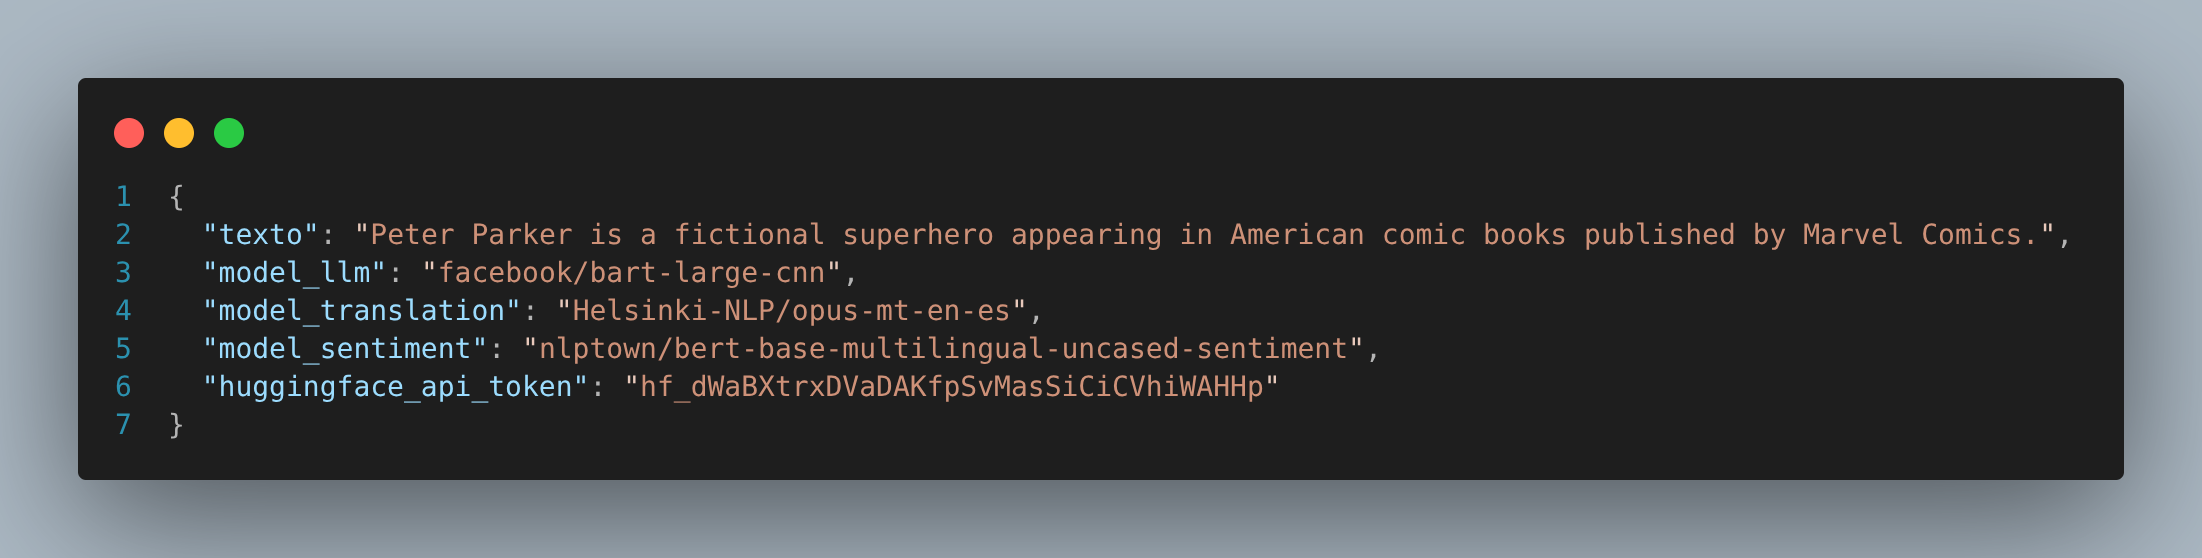
\includegraphics[width=1\linewidth]{./imagenes_necesarias/config_json.png}
				\caption{Contenido del archivo \texttt{config.json}}
				\label{fig:config_json_ej2}
			\end{figure}
			
			Es decir, prácticamente igual que el que se proporciona en la práctica.
			
		\subsection{Diagrama de clases en UML.}
			Tras ver las clases que conforman este proyecto/ejercicio, podemos pasar a ver el diagrama de clases en UML: 
			
			\begin{figure}[H]
				\centering
				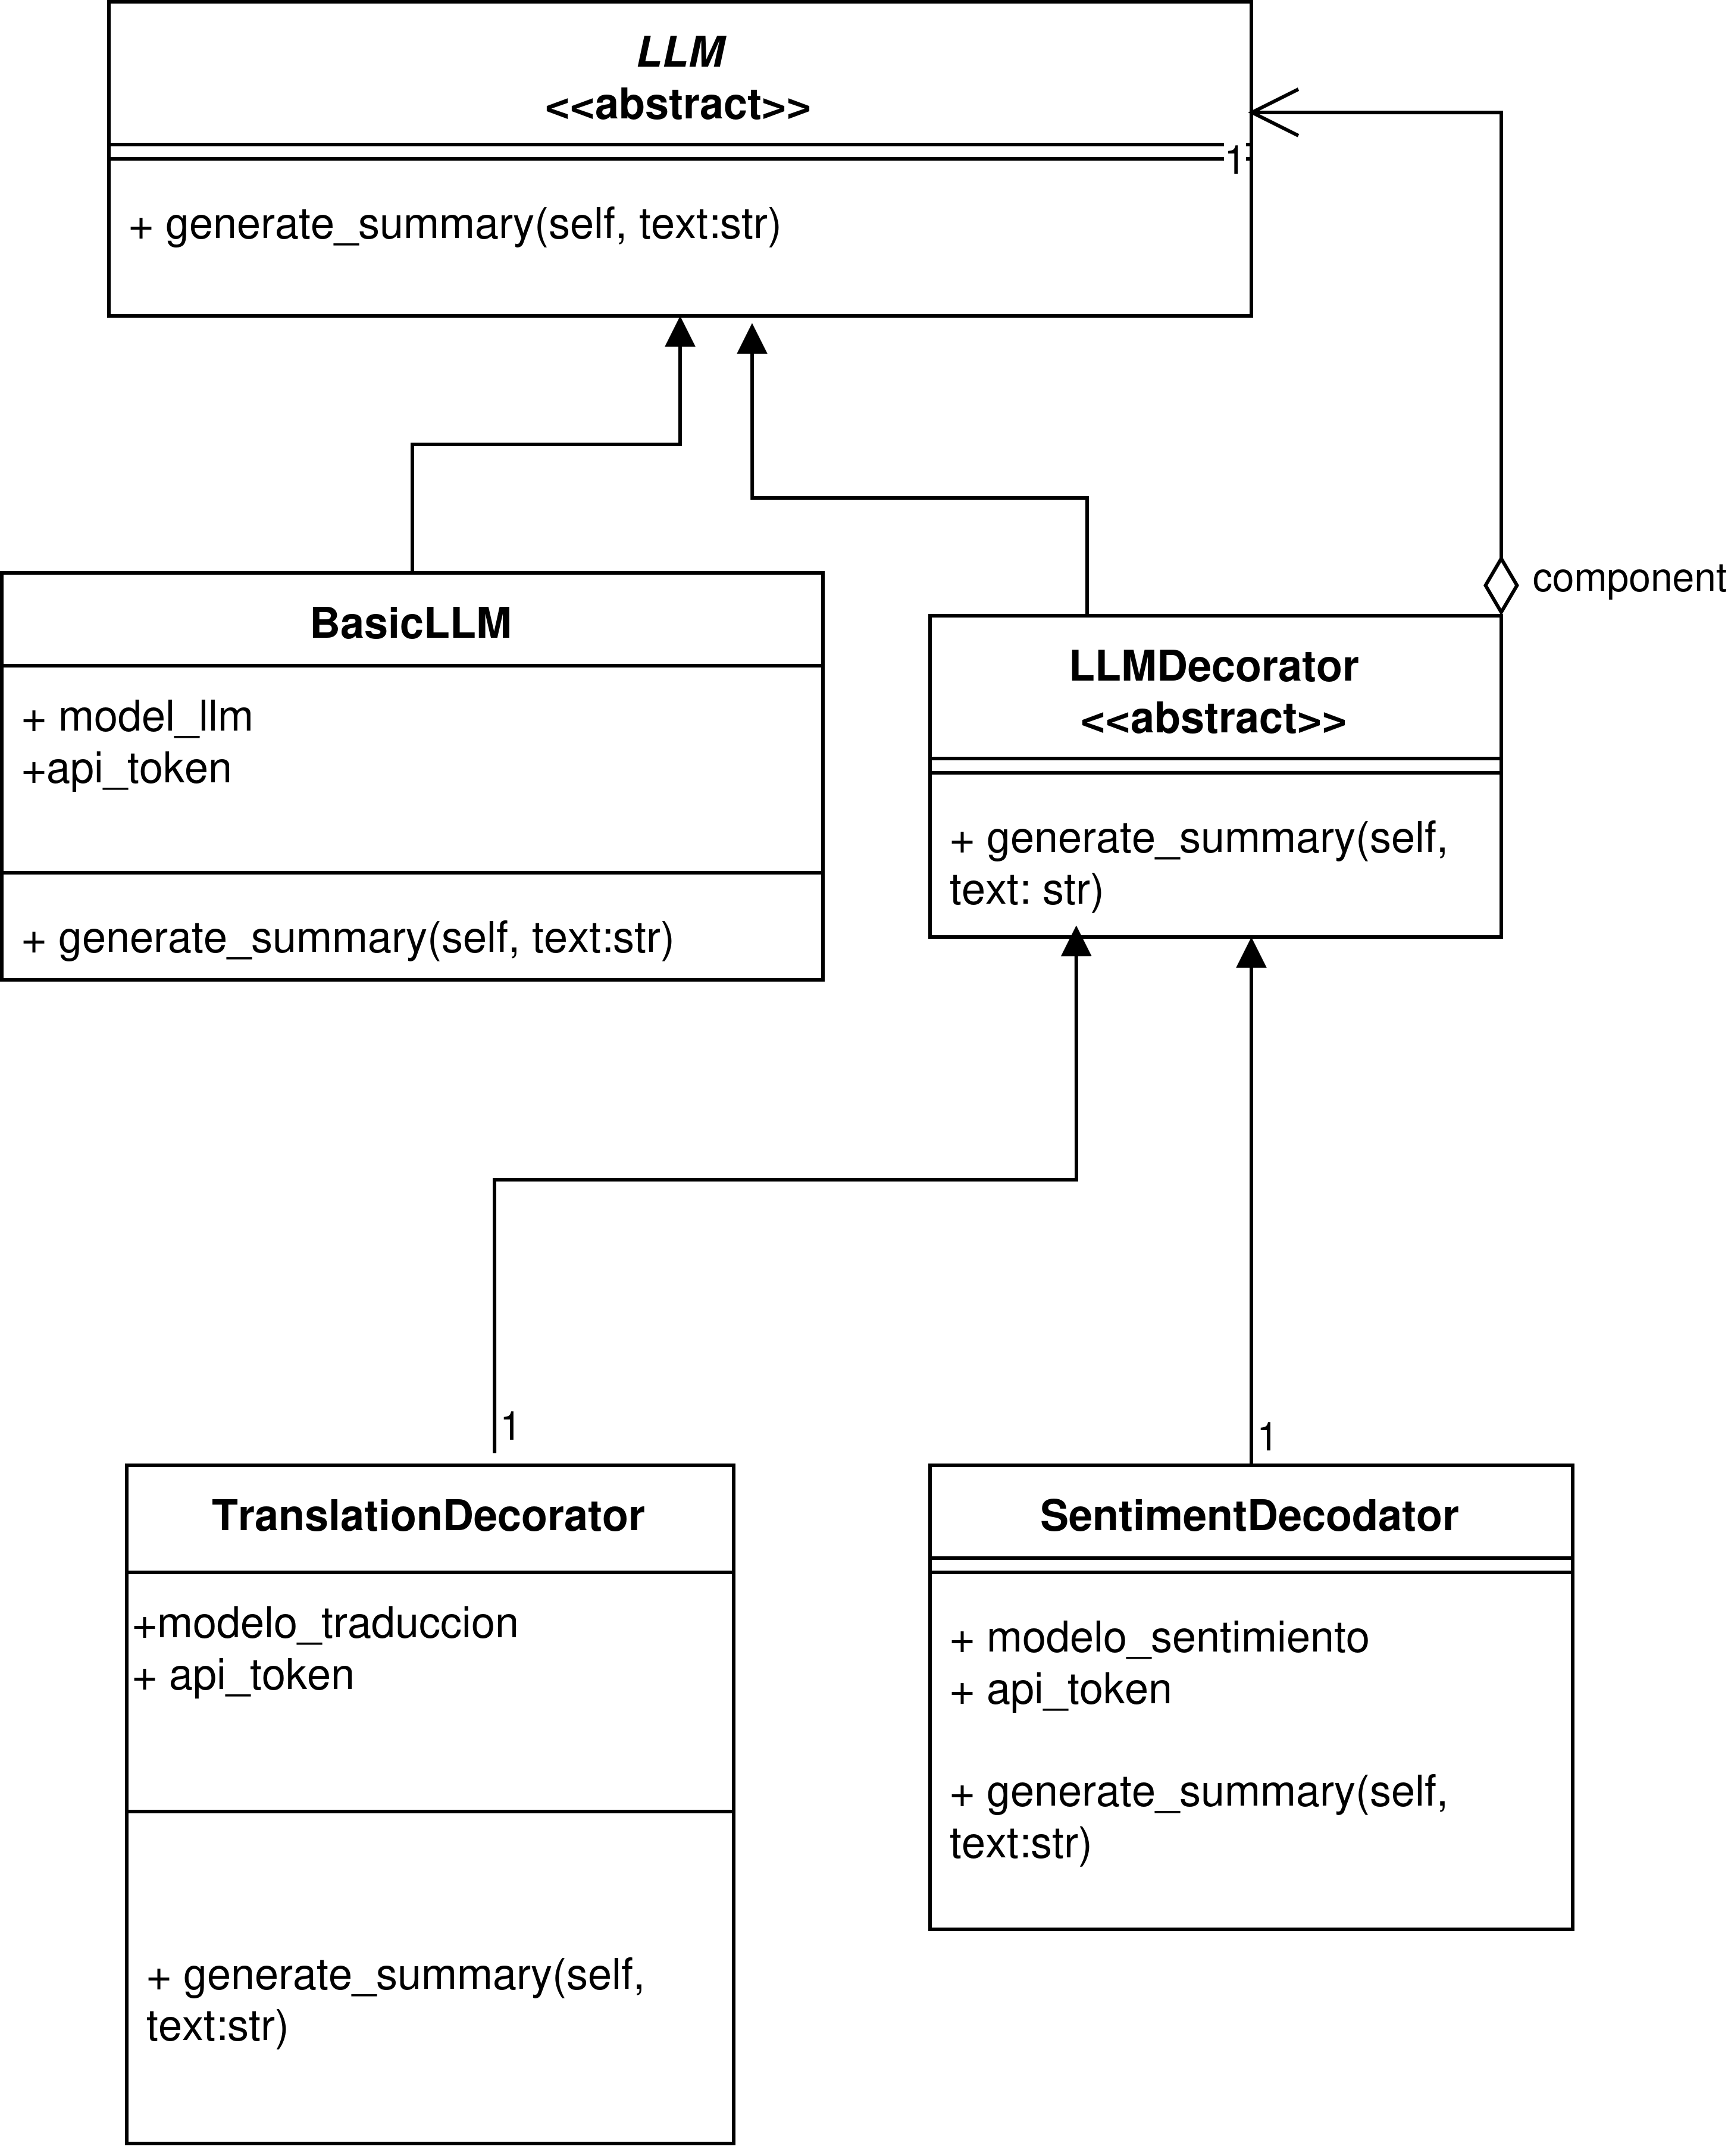
\includegraphics[width=1\linewidth]{../Ejercicio_2_Patron_Decorador_en_Python/diagrama_de_clases/Diagrama_de_clases_EJ2.png}
				\caption{Diagrama de clases del ejercicio 2: Patrón Decorador en Python. }
				\label{fig:dc_ej2}
			\end{figure}
			
		\subsection{Ejemplo de ejecución.}
			Este ejercicio no hace falta compilarlo, pues está hecho en Python y recordemos que es un lenguaje interpretado y no compilado. Entonces, para ejecutar este ejercicio/proyecto simplemente ejecutamos el archivo que hace de función principal, para ello ejecutamos en la terminal el siguiente comando:
			
			\begin{center}
				\fbox{\texttt{\$ python Main.py}}
			\end{center}
			
			A continuación, mostramos una captura de pantalla sobre un ejemplo de ejecución:
			
			\begin{figure}[H]
				\centering
				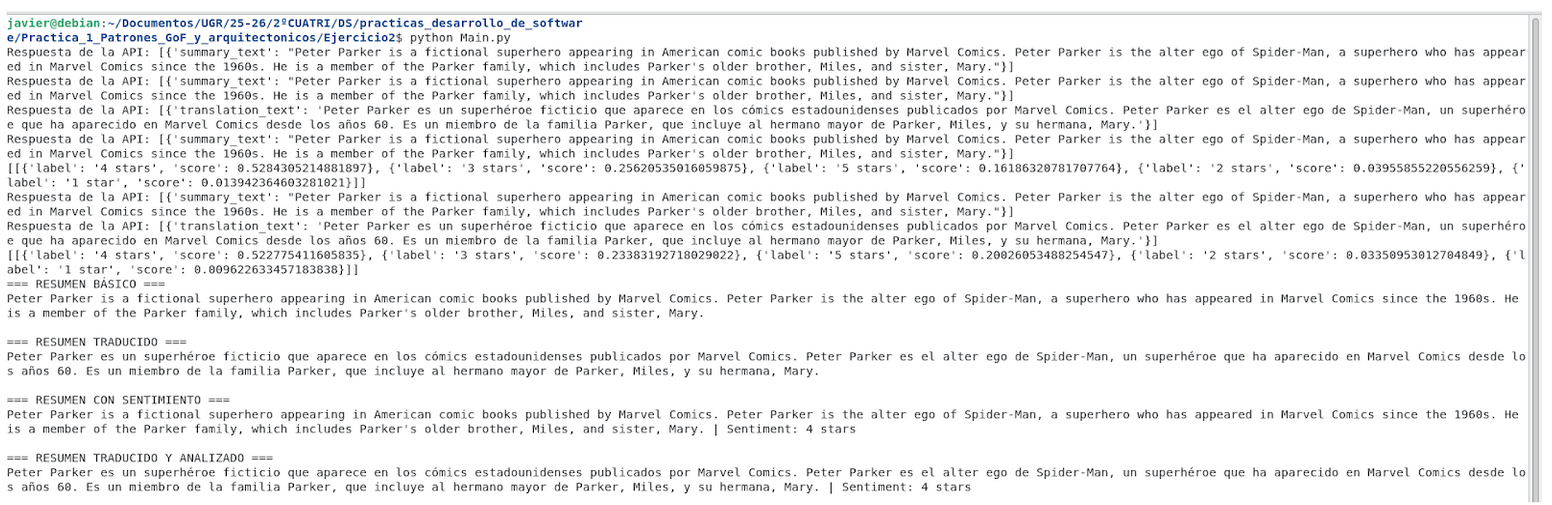
\includegraphics[width=1\linewidth]{./imagenes_necesarias/ejemplo_ejecucion_ej2.png}
				\caption{Ejemplo de ejecución del ejercicio 2.}
				\label{fig:ejemplo_ej2}
			\end{figure}

		\newpage
	
	\section{Ejercicio 3. Patrón Estrategia en Python.}
		El objetivo del ejercicio es aplicar el patrón \textit{Strategy} para permitir seleccionar en tiempo de ejecución (por consola) entre 2 métodos distintos de \textit{web scraping} (obtener info de una página web): uno basado en \texttt{BeautifulSoup} y otro en \texttt{Selenium}, manteniendo desacoplada la lógica del contexto respecto a la implementación concreta. 
		El \textbf{patrón Estrategia (\textit{Strategy})} es un patrón de coportamiento. Los \textbf{patrones de comportamiento} tratan con algoritmos para relacionar la forma en la que los objetos y clases se tratan o interactuan entre sí, repartiéndose responsabilidades. Este patrón Estrategia nos permite definir una familia de algoritmos, encapsularlos y hacerlos intercambiables en tiempo de ejecución según se necesiten.
		
		\subsection{Descripción de elementos del proyecto.}
			\begin{itemize}
				\item \textbf{Interfaz \texttt{ScrapingStrategy}}. Se encuentra en el archivo \texttt{scraping\_strategy.py}. Se trata de una interfaz que define la cabecera del método de extracción de equipos: \mintinline{python}|extract_teams()|, que deberán implementar las clases que implementen esta interfaz.
				
				 \item \textbf{Clase \texttt{HockeyScraperContext}}. Se encuentra en el archivo \texttt{scraping\_context.py} Implementa el \textbf{contexto} que mantiene una referencia a una estrategia y delega en ella la extracción.
				 
				 \item \textbf{Clase \texttt{Beautiful\_Soup}}. Se encuentra en el archivo \texttt{beautifulsoup\_strategy.py}. Esta clase hereda de la clase \texttt{ScrapingStrategy}, y es la  \textbf{estrategia}  que realiza el \textit{scraping} mediante \texttt{request} y \texttt{BeautifulSoup}, recorre las 5 primeras paginas de la web.
				 
				 \item \textbf{Clase \texttt{Selenium}}. Se encuentra en el archivo \texttt{selenium\_strategy.py}. Esta clase hereda de la clase \texttt{ScrapingStrategy}, y realiza el \textit{scraping} automatizando en un navegador sin interfaz gráfica. Hacemos uso del navegador \textbf{Chromium}. 
				 
				 \item \texttt{main.py}.  Cuenta con el \texttt{main}, un método para seleccionar la estrategia en tiempo de ejecución y un método que se encarga de generar y almacenar los datos extraídos en un \texttt{.csv}.
			\end{itemize}
			
			En esta implementación, el \textbf{patrón Estrategia} funcionaría de la siguiente manera:
			
			\begin{itemize}
				\item \textbf{\texttt{ScrapingStrategy}} nos sirve para definir el método común que deberán implementar ambas estrategias. Nos referimos al \mintinline{Python}|método extract_teams()| que se encarga de extraer de cada equipo: Nombre del equipo, Año, Victorias, Derrotas, Derrotas en tiempo extra, Porcentaje de victorias, Goles a favor, Goles en contra y Diferencia de goles. En resumen, nos define el qué, no el cómo. 
				
				\item \textbf{\texttt{HockeyScraperContext}} es el contexto y simplemente delega el trabajo en cualquiera de los estrategias que se seleccionen. ¿Qué aporta entonces el contexto en este caso? Si elimináramos el contexto podríamos hacer funcionar el main haciendo un retoques pero…
				
				\item  El\textbf{ \texttt{main} }decidiría todo, acoplaría estrategias, no sería una buena idea. Por lo que el contexto es esencial para delegar la ejecución del algoritmo en una estrategia concreta (mediante composición) permitiendo intercambiar comportamientos sin necesidad de modificar el código
				
				\item Y por último tenemos las dos posibles estrategias \textbf{\texttt{BeautifulSoupStrategy}} y \textbf{\texttt{SeleniumStrategy}} que implementan dos algoritmos distintos.
			\end{itemize} 
		
		\subsection{Diagrama de clases en UML.}
			El diagrama de clases de este proyecto es el siguiente:
			
			\begin{figure}[H]
				\centering
				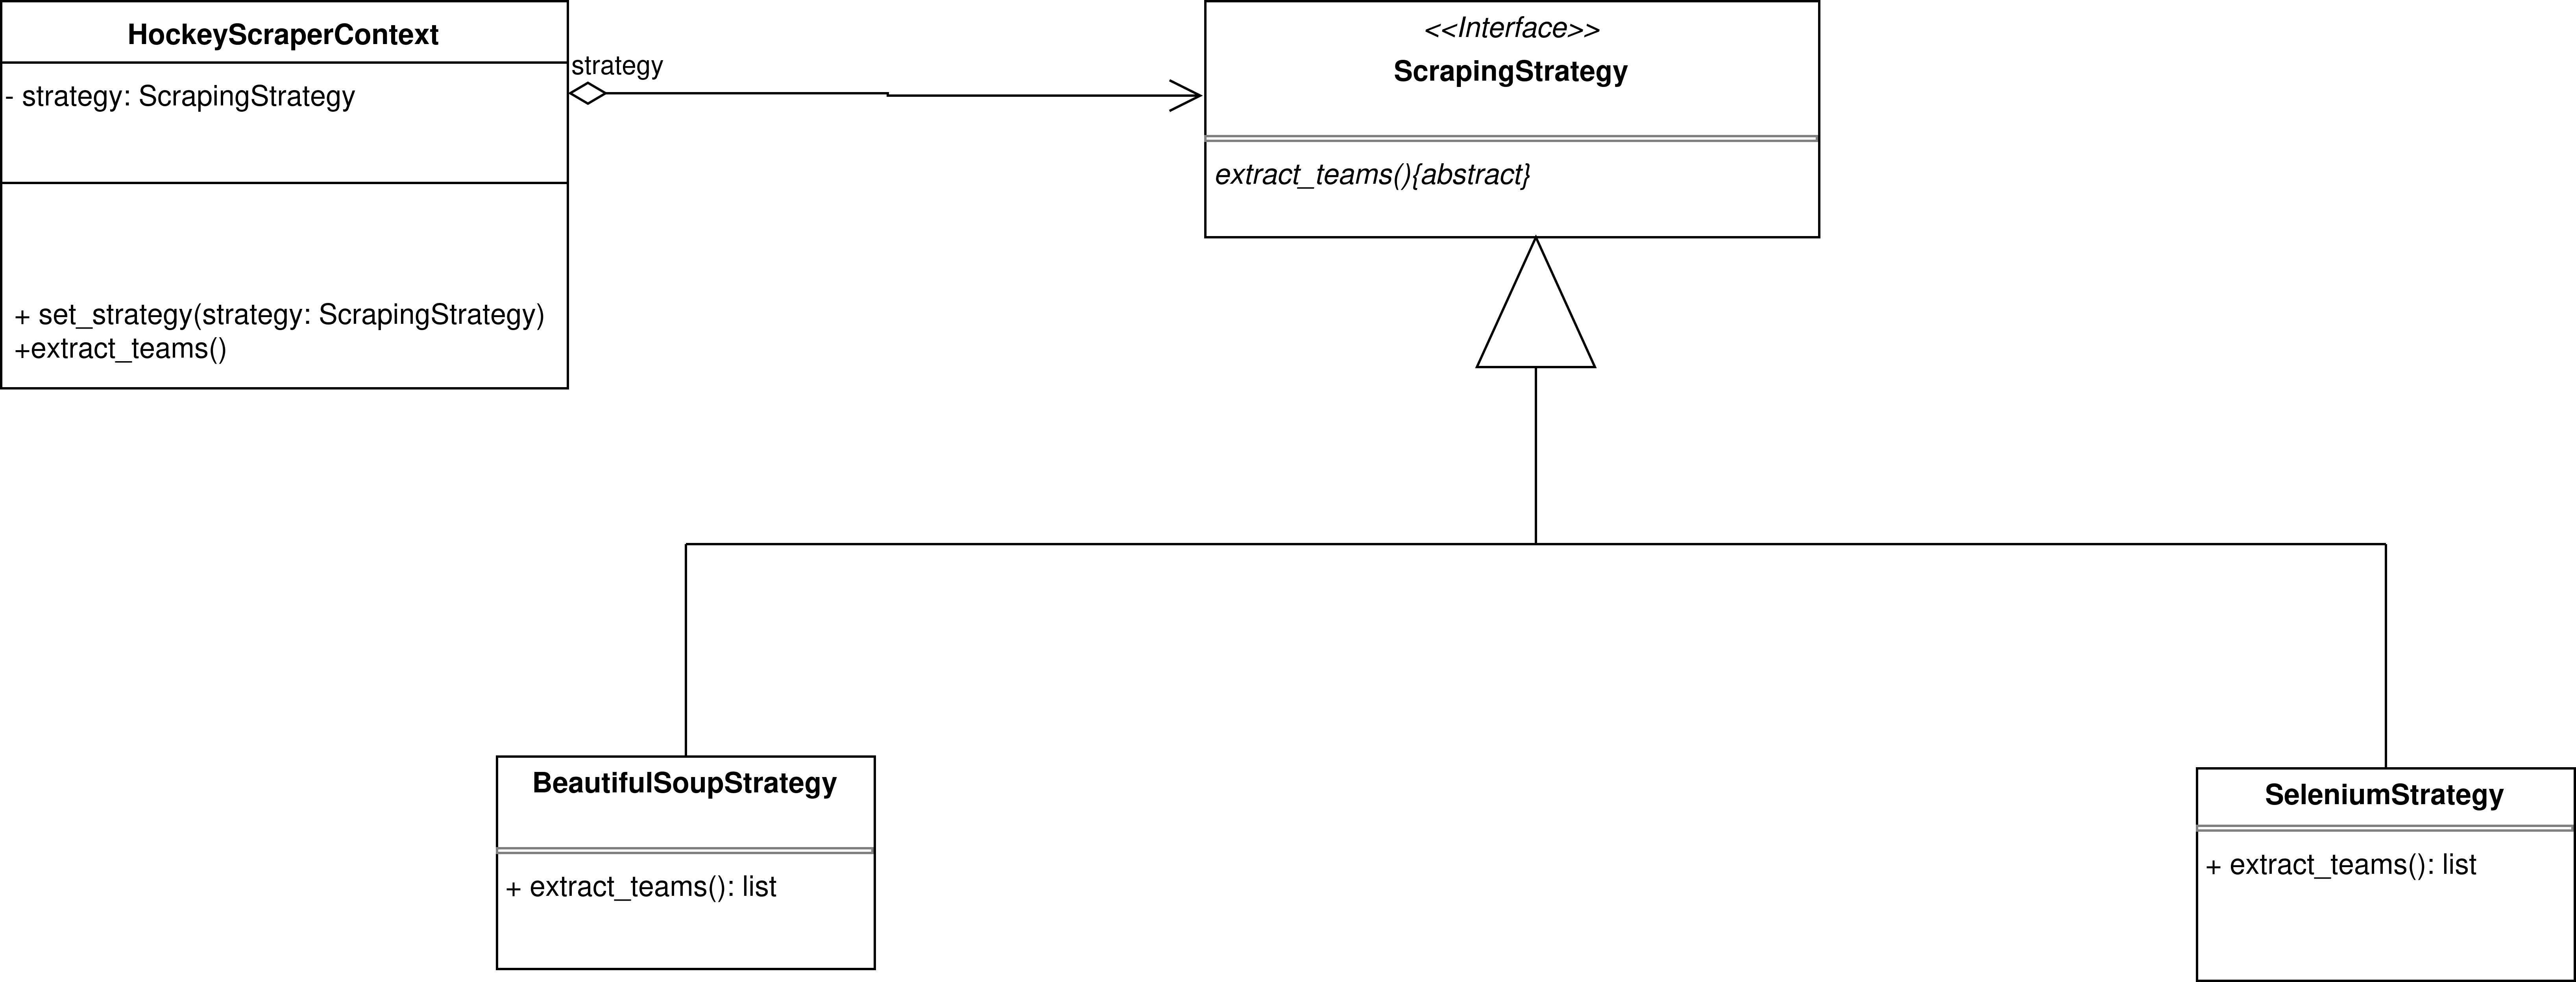
\includegraphics[width=1\linewidth]{../Ejercicio_3_Patron_Estrategia_en_Python/diagrama_de_clases/Diagrama_de_clases_EJ3.png}
				\caption{Diagrama de clases del ejercicio 3: Patrón Estrategia en Python.}
				\label{fig:dc_ej3}
			\end{figure}
			
			\newpage
			
		\subsection{Ejemplos de ejecución.}
			
			Los pasos a seguir para una correcta ejecución son:
			
			\begin{enumerate}
				\item El usuario ejecuta el \texttt{main}. Para ello, ejecutamos en una terminal el siguiente comando:
					\begin{center}
						\fbox{\texttt{\$ python Main.py}}
					\end{center}
					
				\item El programa solicita la estrategia deseada por terminal.
				
				\item  Se crea el objeto estrategia correspondiente.
				
				\item  El contexto llama al método \mintinline{Python}|extract_teams()|.
				
				\item Los datos obtenidos se muestran por pantalla y se guardan en fichero \texttt{CSV}
				
			\end{enumerate}
			
			Aquí presentamos las 2 posibles formas de ejecutar este ejercicio:
			
			\begin{figure}[H]
				\centering
				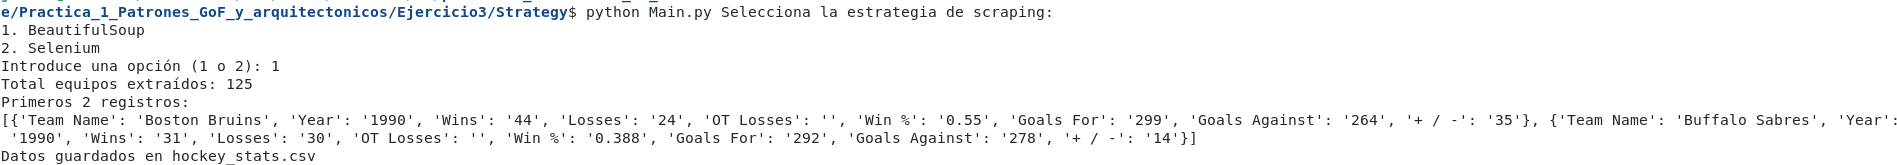
\includegraphics[width=1\linewidth]{./imagenes_necesarias/Ejecución_BS.png}
				\caption{Ejemplo de ejecución del ejercicio 3 usando la estrategia \texttt{BeautifulSoup}.}
				\label{fig:ejemplo1_ej3}
			\end{figure}
			
			\begin{figure}[H]
				\centering
				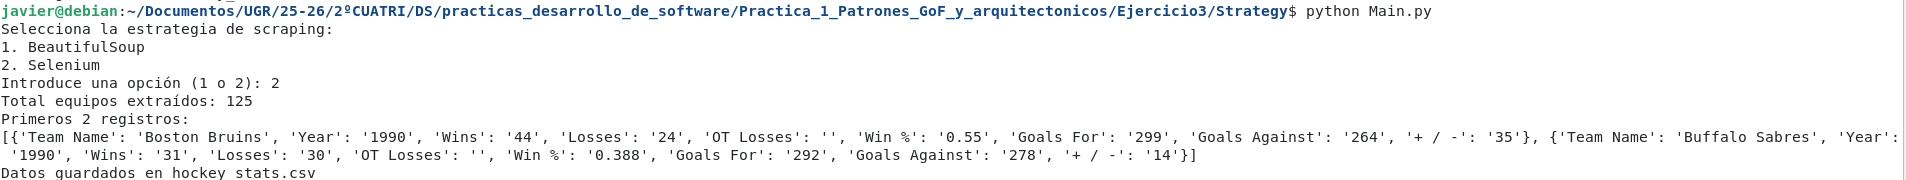
\includegraphics[width=1\linewidth]{./imagenes_necesarias/Ejecución_Selenium.png}
				\caption{Ejemplo de ejecución del ejercicio 3 usando la estrategia \texttt{Selenium}. }
				\label{fig:ejemplo2_ej3}
			\end{figure}
		
			Con ambas estrategias al final del proceso obtenemos un .csv con los datos extraídos de la web. Con 125 elementos, 25 por página, 5 páginas. 
			
			\begin{figure}[H]
				\centering
				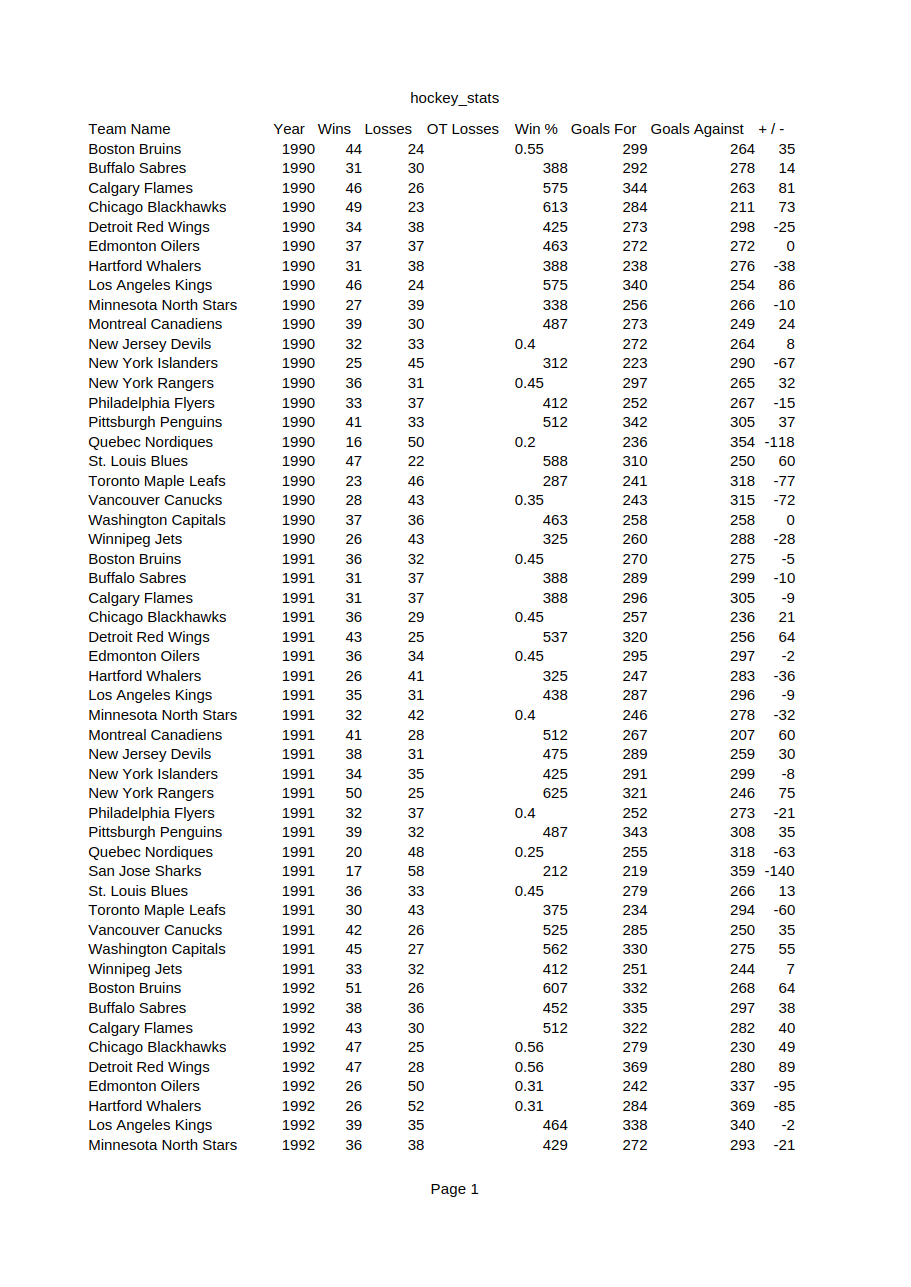
\includegraphics[width=1\linewidth]{./imagenes_necesarias/hockey_stats.png}
				\caption{Contenido del archivo \texttt{hockey\_stats.csv} }
				\label{fig:hs_ej3}
			\end{figure}
		
		\newpage
	
	\section{Ejercicio 4. Patrón filtros de intercepción en Ruby.}
		Este ejercicio trata sobre un servicio de autenticación que requiere validar las credenciales de un usuario, formadas por una dirección de correo electrónico y una contraseña. Además se nos pide que no modifiquemos las clases existenetes y que implementemos el patrón de filtros de intercepción.
		
		El patrón de \textbf{filtros de intercepción} es un patrón de comportamiento. Los\textbf{ patrones conductales (o de comportamiento}) son aquellos que definen la forma de cómo interactúan, se comunican y distribuyen responsabilidades los objetos y clases dentro de un sistema. Este patrón en concreto, sirve para interceptar y manipular una petición antes de que llegue a su destino final (o para modificar la respuesta antes de devolvérsela al cliente), que es lo que buscamos para implementar este servicio de autenticación.
		
		A continuación, vamos a ver los elementos que conforman este ejercicio y que papel juegan dentro de este patrón de diseño.
		
		\subsection{Descripción de elementos del proyecto.}
			\begin{itemize}
				\item \textbf{Clase \texttt{Credenciales}}. Esta clase encapsula las credenciales del usuario, es por eso que sus atributos son el \texttt{correo} y la \texttt{contraseña} del usuario, ambos de tipo \texttt{String}. Además contiene los métodos \texttt{getters} y \texttt{setters} para modificarlos.
				
				\item \textbf{Clase \texttt{Objetivo}}. Esta clase, también conocida como \texttt{target},representa el objetivo a alcanzar si se superan todos los filtros. Sólamente tiene un método que imprime un mensaje por pantalla indicando que se ha alcanzado el objetivo.
				
				\item \textbf{Interfaz \texttt{Filtro}}. Es una interfaz que define la cabecera del método \mintinline{Ruby}|ejecutar(credenciales)|, que todos los filtros que implementen esta interfaz tendrán que implementarlo. Además, la \texttt{Cadena de Filtros} tiene una colección de filtros que son de esta interfaz (aunque ya sabemos que los que implementan este método son los filtros que implementan la interfaz), con ello conseguimos hacer uso de lo que se conoce en POO como \textbf{polimorfismo}.
				
				\item \textbf{Clase \texttt{FiltroPrefijoCorreo}}.Esta clase implementa la interfaz \texttt{Filtro}.  Es el primer filtro que debe pasar el correo introducido por el usuario. Básicamente comprueba que\textbf{ el correo tenga prefijo}, es decir, que tenga texto antes de la \texttt{\@}.
				
				\item \textbf{Clase \texttt{FiltroPrefijoCorreo}}.Esta clase implementa la interfaz \texttt{Filtro}.  Es el segundo filtro que debe pasar el correo introducido por el usuario. Este filtro  comprueba que \textbf{el correo tenga un dominio válido}. Los únicos dominios válidos para este servicio serán \texttt{"gmail.com"} y \texttt{"hotmail.com"}.
				
				\item \textbf{Clase \texttt{FiltroLongitudContrasena}}.Esta clase implementa la interfaz \texttt{Filtro}.  Es el primer filtro que debe pasar la contraseña introducida por el usuario. Comprueba que \textbf{la contraseña tenga como mínimo 8 caracteres}.  
				
				\item \textbf{Clase \texttt{FiltroEspaciosContrasena}}.Esta clase implementa la interfaz \texttt{Filtro}.  Es el segundo filtro que debe pasar la contraseña. Verifica que \textbf{la contraseña no tenga espacio(s) en blanco}.  
				
				\item \textbf{Clase \texttt{FiltroDiferenciaContrasena}}.Esta clase implementa la interfaz \texttt{Filtro}.  Es el tercer filtro que debe pasar la contraseña. Verifica que \textbf{la contraseña y el prefijo del correo sean distintos,} pues de no serlo, la contraseña sería muy débil y el usuario correría un peligro de seguridad.  
				
				\item \textbf{Clase \texttt{CadenaFiltros}}.Esta clase contiene una colección de instancias de las clases anteriores (que implementan los filtros) y una instancia de la clase \texttt{Objetivo}. Es la que está justo por encima de los filtros y del objetivo y por eso es la encargada de gestionarlos, aunque esta clase estará "dirigida" por la siguiente.
				
				\item \textbf{Clase \texttt{GestorFiltros}}. Tal y cómo indica su nombre, esta clase es la encargada de gestionar los filtros (aunque como ya hemos dicho, manda sobre la cadena de filtros, es por eso que tiene un atributo con una instancia de esta clase). Es la encargada de conectar el programa principal (que sería el \texttt{main}), con sus credenciales y los filtros que deben pasar estas últimas. Tiene dos métodos: uno para añadir el filtro que le indique el sistema y lo añade a la cadena de filtros, y otro que realiza una petición de las credenciales pasadas como parámetro (y sobre la que se ejecutarán los filtros).
				
				\item \textbf{Script \texttt{Main}}. Es el programa principal. En él se le pide al usuario que introduzca, por la terminal, su correo y su contraseña. Se crean las credenciales y el objetivo. DEspués se crea el gestor de filtros con el objetivo que acabamos de instanciar. Después, se añaden todos los filtros haciendo uso del método que tiene el gestor de filtros para ello. Y finalmente le indicamos al gestor de filtros que haga una petición con las credenciales que le hemos pasado.
			\end{itemize}
			
		\subsection{Diagrama de clases en UML.}
			El diagrama de clases de este proyecto es el siguiente:
			
			\begin{figure}[H]
				\centering
				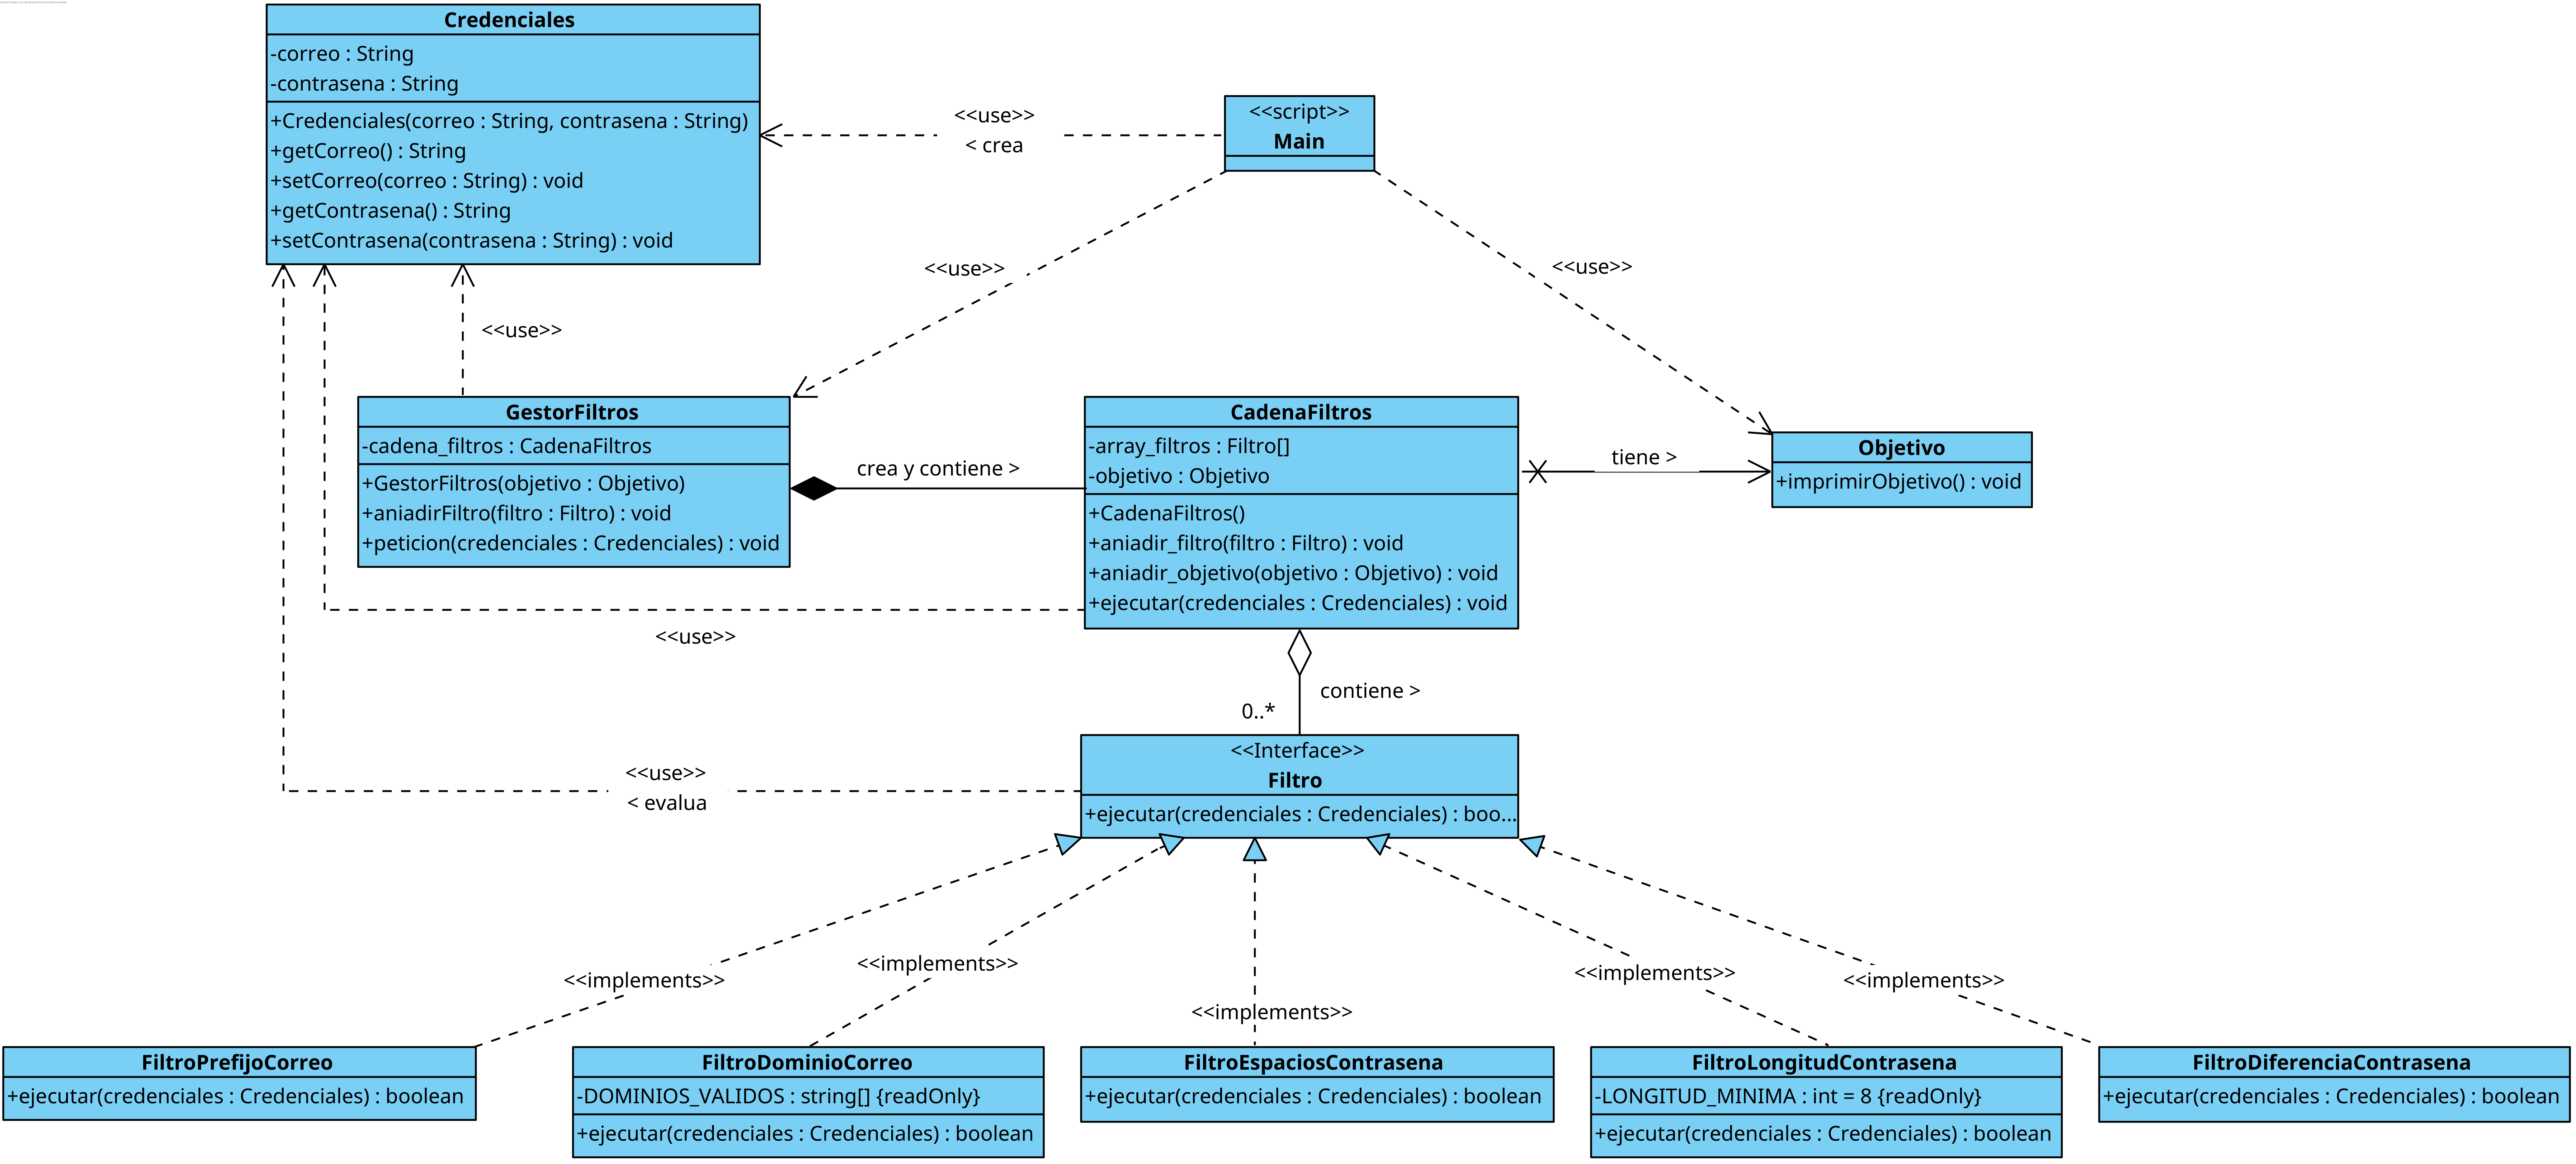
\includegraphics[width=1\linewidth]{../Ejercicio_4_Patron_filtros_intercepcion_en_Ruby/diagramas_UML/Diagrama de Clases1.png}
				\caption{Diagrama de clases del ejercicio 4: Patrón filtros de intercepción en Ruby.}
				\label{fig:dc_ej4}
			\end{figure}
			
			\newpage
			
		
		\subsection{Diagrama de secuencia en UML.}
			En este ejercicio hemos decidido hacer el diagrama de secuencia para ilustrar el funcionamiento de este patrón de diseño, ya que en este diagrama se ve muy bien.
			
			\begin{figure}[H]
				\centering
				\includegraphics[width=1\linewidth]{../Ejercicio_4_Patron_filtros_intercepcion_en_Ruby/diagramas_UML/Diagrama de Secuencia Ejercicio 4 P1 DS.png}
				\caption{Diagrama de secuencia del ejercicio 4: Patrón filtros de intercepción en Ruby.}
				\label{fig:ds_ej4}
			\end{figure}
			
			\newpage
			
		\subsection{Ejemplos de ejecución.}
			
			Para ejecutar este ejercicio simplemente ejecutamos el siguiente comando en la terminal:
			\begin{center}
				\fbox{\texttt{\$ ruby main.rb}}
			\end{center}
			
			A continuación, vamos a ver 5 ejemplos de ejecución con credenciales no válidas para ver como lo detectan los filtros y por último un ejemplo donde las credenciales son válidas y por tanto pasan los filtros y conseguimos el objetivo (que en nuestro sistema será loguearnos).
			
			\begin{itemize}
				\item \textbf{Primer ejemplo}. Filtro del prefijo del correo. Introducimos el correo: \texttt{@gmail.com} y la contraseña: \texttt{software} (aunque daría igual)
				
				\begin{figure}[H]
					\centering
					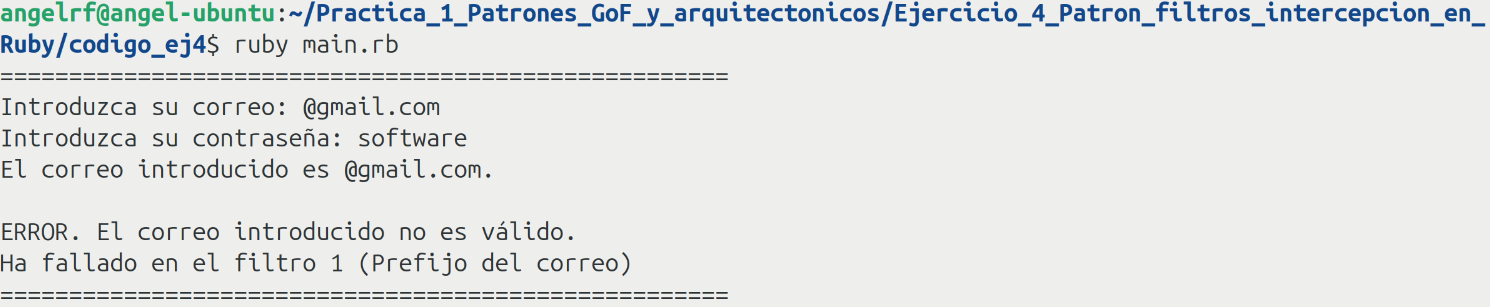
\includegraphics[width=1\linewidth]{./imagenes_necesarias/ejemplo1_ej4.png}
					\caption{Primer ejemplo de ejecución del ejercicio 4.}
					\label{fig:ejemplo1_ej4}
				\end{figure}
				
				\item \textbf{Segundo ejemplo}. Filtro del dominio del correo. Introducimos el correo: \texttt{ingeniero@yahoo.com} y la contraseña: \texttt{software} (aunque daría igual)
				
				\begin{figure}[H]
					\centering
					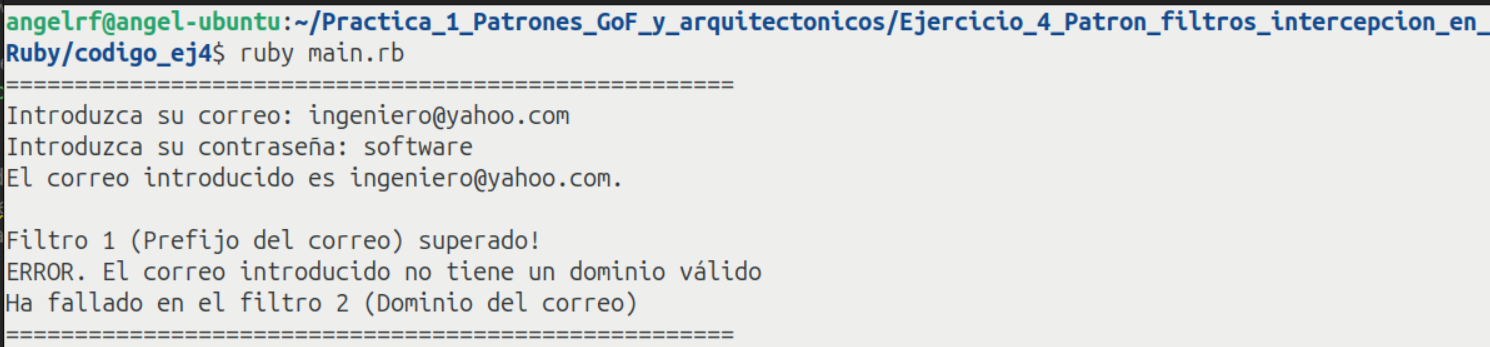
\includegraphics[width=1\linewidth]{./imagenes_necesarias/ejemplo2_ej4.png}
					\caption{Ejemplo de ejecución nº2 del ejercicio 4.}
					\label{fig:ejemplo2_ej4}
				\end{figure}
				
				\item \textbf{Tercer ejemplo}. Filtro de longitud de contraseña. Introducimos el correo: \texttt{ingeniero@gmail.com} y la contraseña: \texttt{soft}
				
				\begin{figure}[H]
					\centering
					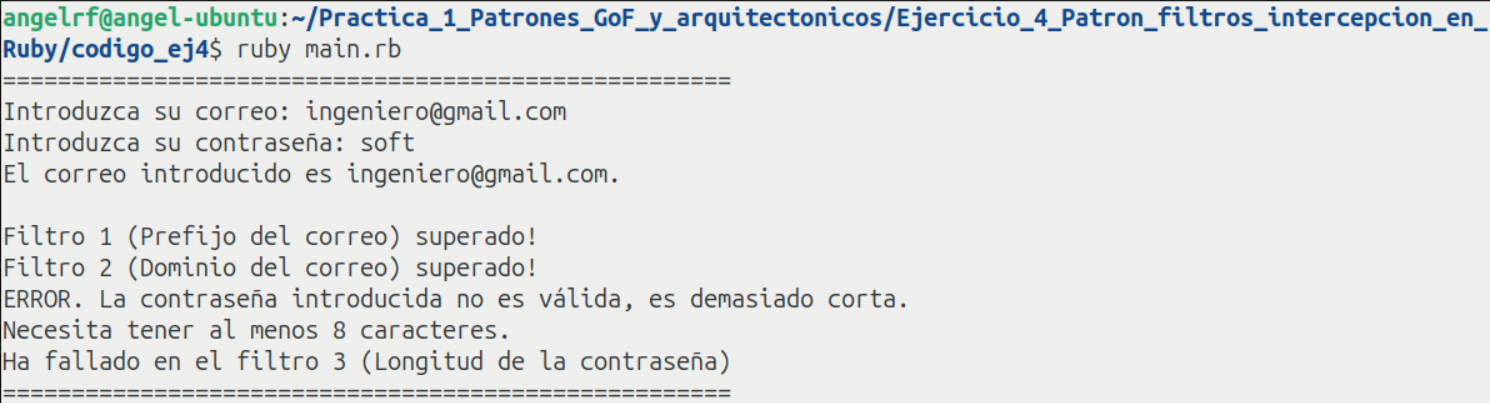
\includegraphics[width=1\linewidth]{./imagenes_necesarias/ejemplo3_ej4.png}
					\caption{Ejemplo de ejecución nº3 del ejercicio 4.}
					\label{fig:ejemplo3_ej4}
				\end{figure}
				
				\item \textbf{Cuarto ejemplo}. Filtro de espacios de contraseña. Introducimos el correo: \texttt{ingeniero@gmail.com} y la contraseña: \texttt{soft wa re}
				
				\begin{figure}[H]
					\centering
					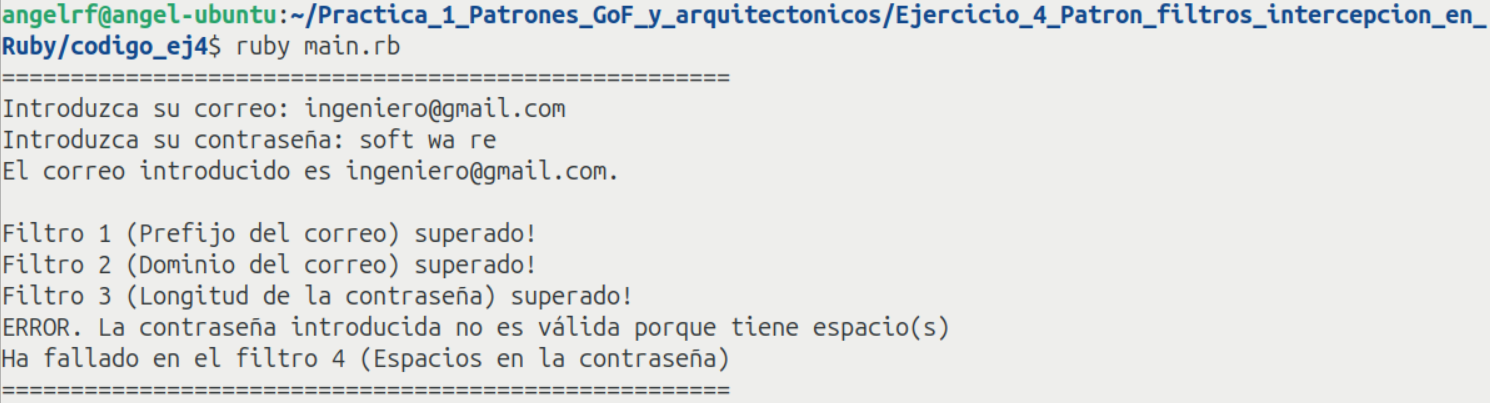
\includegraphics[width=1\linewidth]{./imagenes_necesarias/ejemplo4_ej4.png}
					\caption{Ejemplo de ejecución nº4 del ejercicio 4.}
					\label{fig:ejemplo4_ej4}
				\end{figure}
				
				\item \textbf{Quinto ejemplo}. Filtro de diferencia de contraseña. Introducimos el correo: \texttt{ingeniero@gmail.com} y la contraseña: \texttt{ingeniero}
				
				\begin{figure}[H]
					\centering
					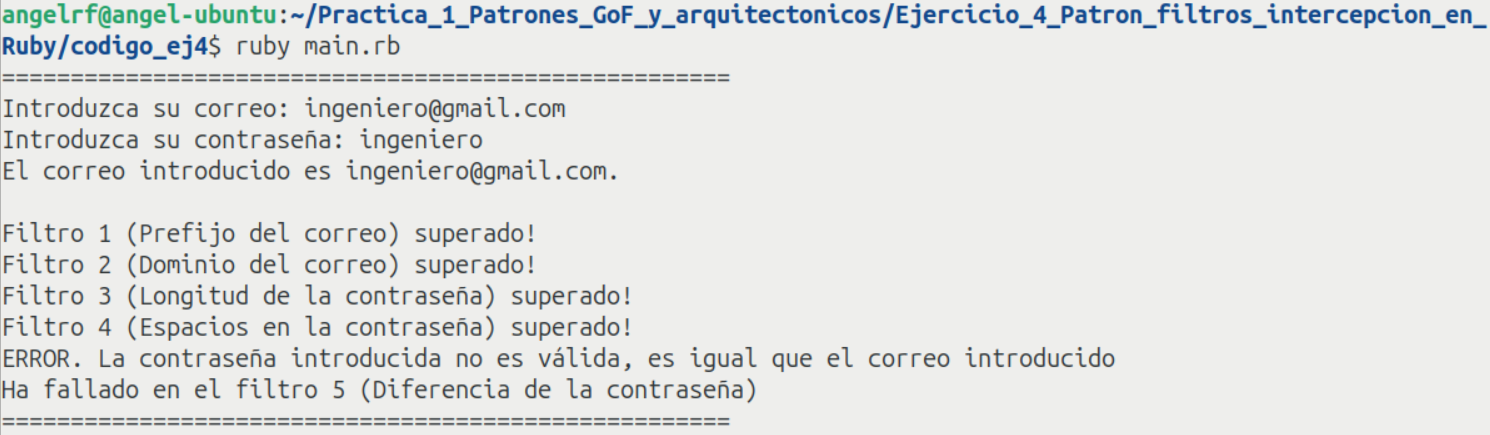
\includegraphics[width=1\linewidth]{./imagenes_necesarias/ejemplo5_ej4.png}
					\caption{Ejemplo de ejecución nº5 del ejercicio 4.}
					\label{fig:ejemplo5_ej4}
				\end{figure}
				
				\item \textbf{Sexto ejemplo}. Credenciales correctas. Introducimos el correo: \texttt{ingeniero@gmail.com} y la contraseña: \texttt{software}
				
				\begin{figure}[H]
					\centering
					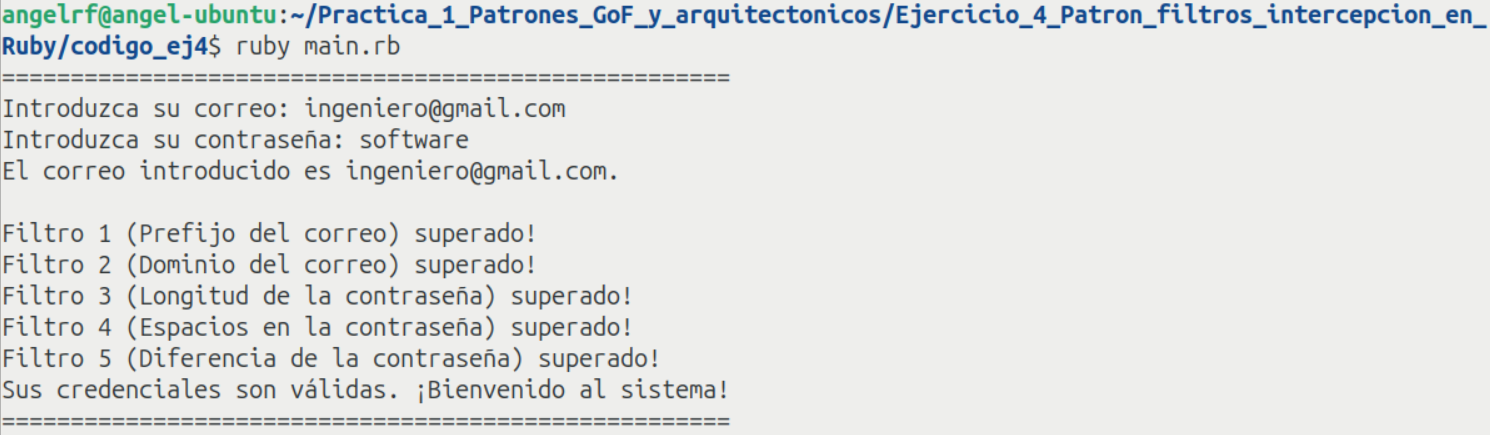
\includegraphics[width=1\linewidth]{./imagenes_necesarias/ejemplo6_ej4.png}
					\caption{Ejemplo de ejecución nº6 del ejercicio 4.}
					\label{fig:ejemplo6_ej4}
				\end{figure}
				
				
			\end{itemize}

	
\end{document}